\documentclass[a4paper, 10pt, twocolumn, titlepage]{article}

\usepackage{verbatim}
\usepackage{xcolor}
\usepackage{indentfirst}
\usepackage{cite}
\usepackage{lipsum}
\usepackage[margin=25mm]{geometry}
\usepackage{amsmath}
\usepackage{nth}
\usepackage{hyperref}
\usepackage[us,12hr]{datetime} % `us' makes \today behave as usual in TeX/LaTeX
\usepackage{booktabs}
\usepackage[font=small,labelfont=bf]{caption}
\usepackage{graphicx} % for pdf, bitmapped graphics files
\graphicspath{{./fig/}}
\DeclareGraphicsExtensions{.pdf,.jpeg,.png}
\usepackage{subfigure}

\newcommand{\head}[1]{\textnormal{\textbf{#1}}} % for tables

\title{CRIM Surya University: Flapping bird robot project \\ Electrical and Electronics Specifications }

\author{Vektor Dewanto\footnote{vektor.dewanto at gmail.com; compiled on {\ddmmyyyydate\today} at \currenttime}}
\date{\today}

\hyphenation{lay-out se-pa-ra-te}

\begin{document}
\maketitle
\tableofcontents

%%%%%%%%%%%%%%%%%%%%%%%%%%%%%%%%%%%%%%%%%%%%%%%%%%%%%%%%%%%%%%%%%%%%%%%%%%%%%%%%
\section{Introduction}
This document presents electrical and electronics specifications for the flapping bird robot (ornithopter) project.
The high level block diagram of the proposed system is shown in figure~\ref{fig:hi-level_diagram}.

\begin{figure*}[!tb]
  \centering
  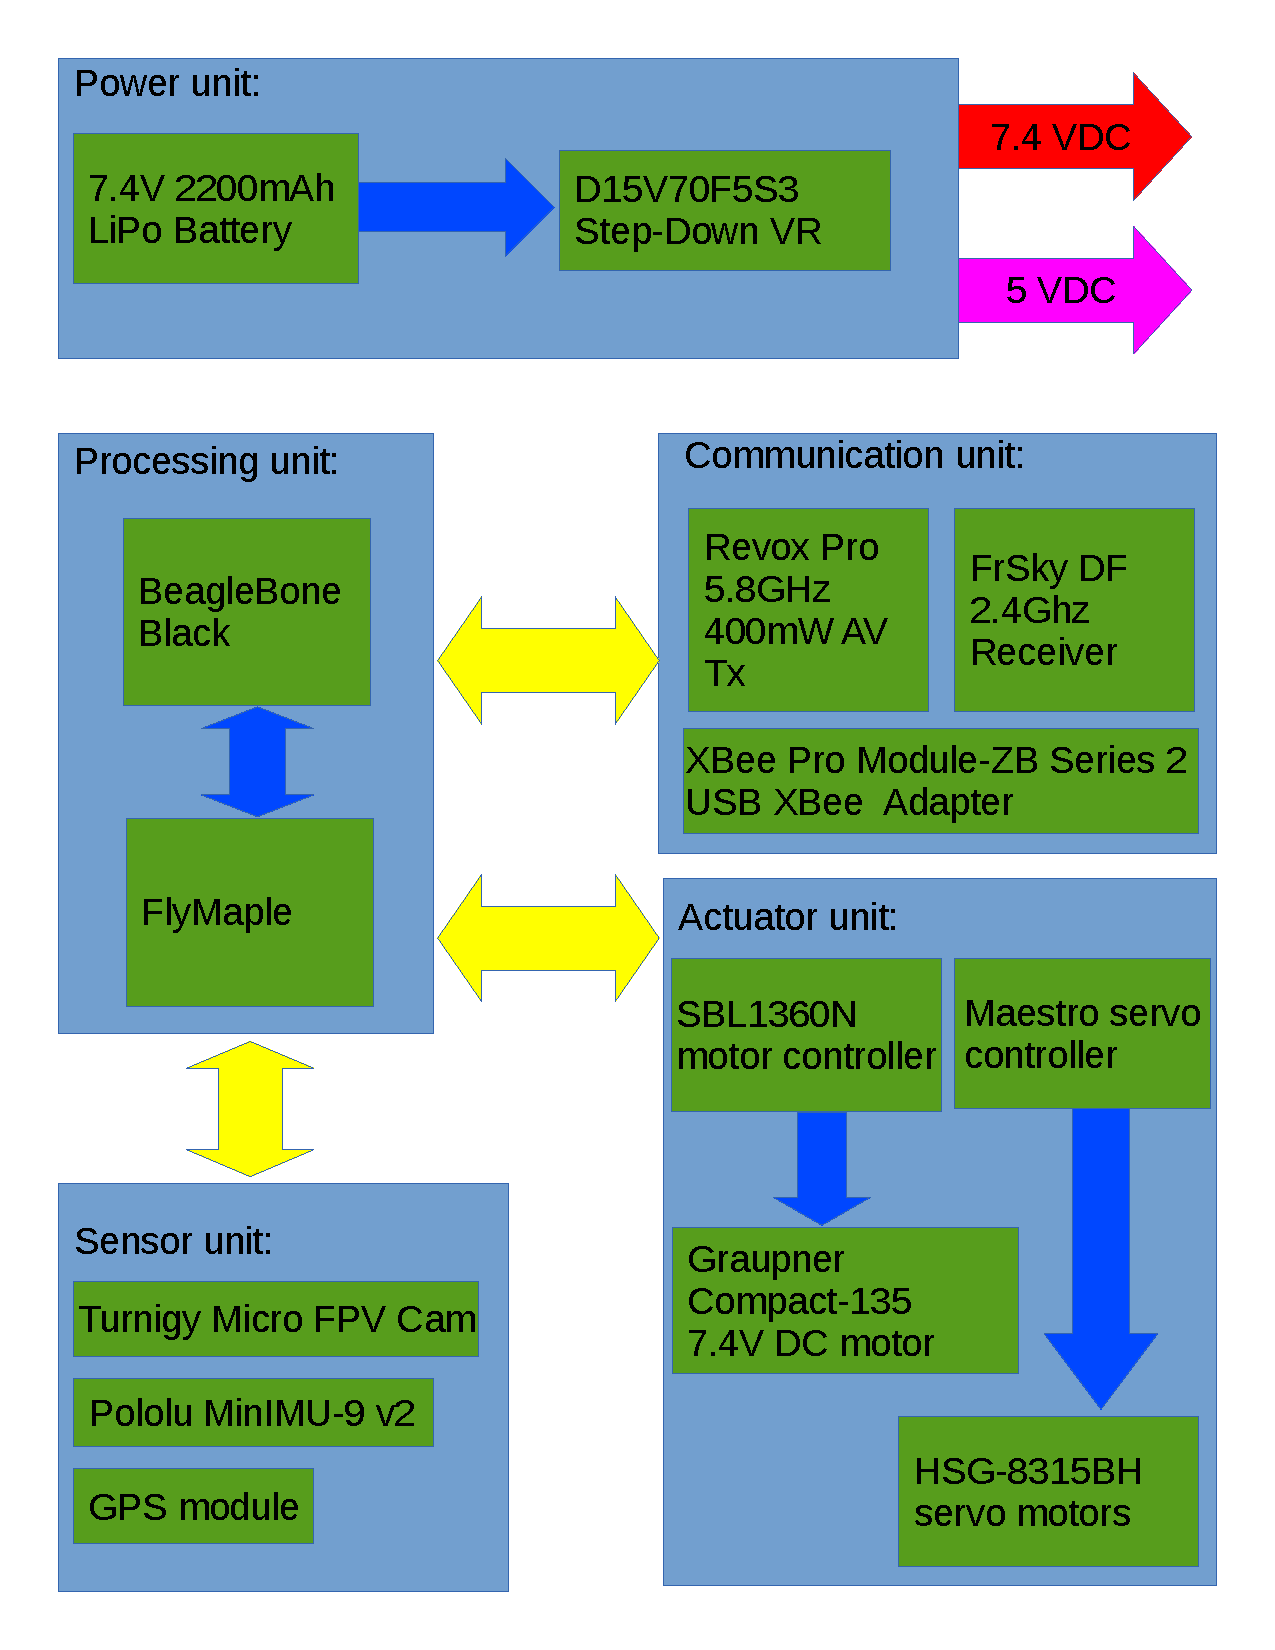
\includegraphics[scale=.50]{hi-level_diagram}
  \caption{The high level block diagram of the proposed system.}
  \label{fig:hi-level_diagram}
\end{figure*}

We remark that the best reference model thus far is the SmartBird project from FESTO, which was revealed in 2011.
Other noticeble projects include the Big Bird Robo Raven (University of Maryland), the RoboSwift (Delft University of Technology) and the Bat robots (Brown University).
Besides, some (toy) ornithopter products are worth attention, such as  WowWee Flytech Dragonfly, Cybird 2-Channel RC Ornithopter and E-Bird Flapping-Wing Aircraft R/C Flying Robot and Avitron V2.0.

%%%%%%%%%%%%%%%%%%%%%%%%%%%%%%%%%%%%%%%%%%%%%%%%%%%%%%%%%%%%%%%%%%%%%%%%%%%%%%%%
\section{Management}
\subsection{Work Breakdown Structure}
\begin{enumerate}
\itemsep-0.5mm
  \item Electronics
    \begin{enumerate}
    \itemsep-0.5mm
      \item Design  \label{wbs:ee_design}
      \item Purchasing \label{wbs:ee_purchasing}
      \item Communication  \label{wbs:ee_comm}
        \begin{enumerate}
        \itemsep-0.5mm
          \item Data commmunication
          \item Control communication
        \end{enumerate}
      \item Sensor \label{wbs:ee_sensor}
        \begin{enumerate}
        \itemsep-0.5mm
          \item Inertial measurement unit
          \item Webcam
          \item GPS
        \end{enumerate}
      \item Actuator  \label{wbs:ee_actuator}
        \begin{enumerate}
        \itemsep-0.5mm
          \item BLDC motor control
          \item Servo motor control
        \end{enumerate}
      \item Power  \label{wbs:ee_pwr}
        \begin{enumerate}
        \itemsep-0.5mm
          \item Battery and charging
          \item Power regulation and monitoring
        \end{enumerate}
      \item Integration
        \begin{enumerate}
        \itemsep-0.5mm
          \item EE-only integration  \label{wbs:ee_int}
          \item EE and ME integration \label{wbs:ee-me_int}
        \end{enumerate}
    \end{enumerate}
  \item Control systems
    \begin{enumerate}
    \itemsep-0.5mm
      \item Design \label{wbs:ctrl_design}
        \begin{enumerate}
        \itemsep-0.5mm
          \item Open study
          \item Reinforcement learning study
          \item Experiment design
        \end{enumerate}
      \item Implementation \label{wbs:ctrl_impl}
        \begin{enumerate}
        \itemsep-0.5mm
          \item Reinforcement learning experiments
          \item Mechanical System Identification
        \end{enumerate}
      \item Tests \label{wbs:ctrl_test}
        \begin{enumerate}
        \itemsep-0.5mm 
          \item Straight flight
          \item Up-and-down flight 
          \item Curvy flight
          \item Gliding flight
        \end{enumerate}
    \end{enumerate}
  \item Closure
    \begin{enumerate}
    \itemsep-0.5mm
      \item Demonstrations  \label{wbs:demo}
      \item Reports  \label{wbs:rpt}
    \end{enumerate}
\end{enumerate}

\subsection{Schedule}
The timeline is shown in table~\ref{tbl:gantt-chart}.

\begin{table*}[!tb]
\centering
\caption{The gantt chart}
  \begin{tabular}{l cccc cccc cccc cccc cccc}
    \toprule[1.5pt]
    
    \multicolumn{1}{c}{\head{WBS}} &
    \multicolumn{4}{c}{\head{Nov}} &
    \multicolumn{4}{c}{\head{Dec}} &
    \multicolumn{4}{c}{\head{Jan}} &
    \multicolumn{4}{c}{\head{Feb}} &
    \multicolumn{4}{c}{\head{Mar}} \\
    
    & \head{1} & \head{2} & \head{3} & \head{4} &
      \head{1} & \head{2} & \head{3} & \head{4} &
      \head{1} & \head{2} & \head{3} & \head{4} &
      \head{1} & \head{2} & \head{3} & \head{4} &
      \head{1} & \head{2} & \head{3} & \head{4} \\
    
    \cmidrule(r){1-1} \cmidrule(l){2-5} \cmidrule(l){6-9} \cmidrule(l){10-13} \cmidrule(l){14-17} \cmidrule(l){18-21}
    
    \ref{wbs:ee_design}: ee design &
     X & X & X &   &
       &   &   &   &
       &   &   &   &
       &   &   &   &
       &   &   &   \\
     
    \ref{wbs:ee_purchasing}: ee purchasing &
       &   & X & X &
     X &   &   &   &
       &   &   &   &
       &   &   &   &
       &   &   &   \\
    
    \midrule[1.0pt]
    \ref{wbs:ee_comm}: ee comm &
       &   &   &   &
     X &   &   &   &
       &   &   &   &
       &   &   &   &
       &   &   &   \\
    
    \ref{wbs:ee_sensor}: ee sensor &
       &   &   &   &
     X &   &   &   &
       &   &   &   &
       &   &   &   &
       &   &   &   \\
    
    \midrule[1.0pt]
    \ref{wbs:ee_actuator}: ee actuator &
       &   &   &   &
       & X &   &   &
       &   &   &   &
       &   &   &   &
       &   &   &   \\
    
    \ref{wbs:ee_pwr}: ee power &
       &   &   &   &
       & X &   &   &
       &   &   &   &
       &   &   &   &
       &   &   &   \\
    
    \midrule[1.0pt]
    \ref{wbs:ee_int}: ee intgr &
       &   &   &   &
       &   & X & X &
       &   &   &   &
       &   &   &   &
       &   &   &   \\
       
    \ref{wbs:ee-me_int}: ee-me intgr &
       &   &   &   &
       &   &   & X &
     X & X &   &   &
       &   &   &   &
       &   &   &   \\

    \midrule[1.0pt]
    \ref{wbs:ctrl_design}: ctrl design &
       &   & X & X &
     X & X & X & X &
     X & X &   &   &
       &   &   &   &
       &   &   &   \\

    \ref{wbs:ctrl_impl}: ctrl impl &
       &   &   &   &
       &   &   &   &
       & X & X & X &
     X & X &   &   &
       &   &   &   \\
    
    \ref{wbs:ctrl_test}: ctrl test &
       &   &   &   &
       &   &   &   &
       &   &   &   &
       & X & X & X &
     X & X & X &   \\
              
    \midrule[1.0pt]
    \ref{wbs:rpt}: reports &
       &   &   &   &
       &   &   &   &
       &   &   &   &
       &   &   &   &
       &   & X & X \\

    \ref{wbs:demo}: demo &
       &   &   &   &
       &   &   &   &
       &   &   &   &
       &   &   &   &
       & X &   & X \\
                     
    \bottomrule[1.5pt]
  \end{tabular}
\label{tbl:gantt-chart}
\end{table*}

\subsection{Milestones}
\begin{enumerate}
  \item \emph{Milestone-1 (Dec: Week-3)} ee-only integration
  \item \emph{Milestone-2 (Jan: Week-3)} ee-me integration
  \item \emph{Milestone-3 (Feb: Week-3)} first trial
  \item \emph{Milestone-4 (Mar: Week-2)} first demo
  \item \emph{Milestone-5 (Dec: Week-4)} hand-off
\end{enumerate}
    
%%%%%%%%%%%%%%%%%%%%%%%%%%%%%%%%%%%%%%%%%%%%%%%%%%%%%%%%%%%%%%%%%%%%%%%%%%%%%%%%
\section{Hardware}
This section lists all hardware that is \emph{on-board} on the robot body.
For procurement information, refer to section~\ref{sec:procurement}.
For the summary of dimensions and weights, refer to table~\ref{tbl:hw_dim_weight}.

\begin{table*}[!tb]
\centering
\caption{Hardware dimensions (milimeters) and weights (grams)}
  \begin{tabular}{llr}
    \toprule[1.5pt]
    \head{Type} & \head{Dimensions} & \head{Weight} \\
    \toprule[1.0pt]
    
    %%%
    BeagleBone Black and or FlyMaple & 
    86.36 x 53.34 x 4.76 & 
    39.68 \\
    
    %%%
    \midrule
    XBee Pro Module - ZB Series 2 & 
    24.00 x 33.00 x 9.00 & 
    3.91 \\
    
    USB XBee Adapter & 
    38.30 x 25.60 x 14.80 & 
    4.00 \\
    
    FrSky DF 2.4Ghz Receiver & 
    55 x 25 x 14 & 
    12.4 \\
    
    Revox Pro 5.8GHz 400mW AV Tx &
    55.00 x 26.00 x 17.00 &
    52.00 \\
    
    %%%
    \midrule
    MinIMU-9 v2 &
    20.00 x 13.00 x 3.00 & 
    0.70 \\
    
    Turnigy Micro FPV Camera &
    34.00 x 34.00 x 30.00 & 
    40.00 \\
    
    Adafruit v3 GPS &
    25.50 x 35.00 x 6.50 & 
    8.50 \\
    
    %%%
    \midrule
    Turnigy Park300 BLDCM &
    27.00 x 23.00 & 
    25.00 \\
    
    Hitec HS-82MG Micro Servo &
    30 x 30 x 12 & 
    19.00 \\
    
    20A BlueSeries ESC &
    33 x 23 x 6 & 
    18.00 \\
    
    Micro Maestro Servo Controller &
    21.59 x 30.48 x 6.00 & 
    4.80 \\
    
    %%%
    \midrule
    7.4V 2200mAh Turnigy Lipo Battery  &
    12 x 35 x 18  & 
    133.00 \\
  
    D15V70F5S3 Step-Down VR &
    48.00 x 15.00 x 8.00 & 
    6.00 \\
    
    ACS715 Current Sensor &
    17.78 x 20.32 &
    1.30 \\
    
    %%%
    \midrule
    Cables and connectors  &
    n.a & 
    1.00 \\
    
    %%%
    \midrule
    TOTAL  &
    n.a &  
    369.29 \\
        
    \bottomrule[1.5pt]
  \end{tabular}
\label{tbl:hw_dim_weight}
\end{table*}

\subsection{Processing units}
We employ a BeagleBone Black as the main processing unit.
It uses an AM335x 1GHz ARM® Cortex-A8 processor.
Its key specifications are as follows:
\begin{itemize}
\itemsep-1mm 
  \item  512MB DDR3 RAM
  \item  2GB 8-bit eMMC on-board flash storage
  \item  3D graphics accelerator
  \item  NEON floating-point accelerator
  \item  2x PRU 32-bit microcontrollers
  \item  compatible with  \AA ngstrom, Android, Ubuntu
  \item  USB client for power and communications
  \item  USB host, Ethernet, HDMI, 2 x 46 pin headers
  \item  dimensions: 86.36mm x 53.34mm x 4.76mm
  \item  weight: 39.68 grams
\end{itemize}

As an alternative (and probably a complement), we use one Flymaple, which is a Quadcopter controller board based on the Maple Project.
Its specifications include:
\begin{itemize}
  \itemsep-1mm
  \item Microcontroller: STM32F103
  \item Running at 72Mhz with 32bit Arduino sytle ARM processor(Cortex-M3)
  \item ITG-3200 - triple-axis digital-output gyroscope
  \item ADXL345 - 13-bit resolution, ±16g, triple-axis accelerometer
  \item HMC5883L - triple-axis, digital magnetometer
  \item BMP085 - high-precision barometric pressure sensor
  \item Programable through an Arduino-based development environment - Maple IDE
  \item Extends 6 channels PWM pins for controlling ESC/Servo
  \item Extends 8 channels GPIO for capturing RC receiver output
  \item Serial port 1
  \item GPS extension port
  \item I2C interface
  \item Size: 50x50x12mm
  \item Weight: 15g
\end{itemize}

\subsection{Communication units}
\subsubsection{Data communication}
This communication channel is mainly used for data (images, measurement results) acquisition to the ground, not for flight control signals.
For the latter, refer to subsubsection~\ref{subsec:ctrl_comm}.

The wireless communication for measurement (sensing) data is based on Zigbee protocol.
In particular, we use an XBee Pro Module ZB Series 2.
Its technical details are as follows:
\begin{itemize}
\itemsep-1mm
  \item  TX Peak Current: 205mA
  \item  RX Current: 47 mA (@3.3 V)
  \item  power-down Current: $< 3.5 \mu A$
  \item  indoor/Urban: up to 300 ft (90 m)
  \item  outdoor line-of-sight: up to 2 miles (3200 m)
  \item  transmit Power: 63mW (18dBm)
  \item  receiver Sensitivity: -102 dBm
  \item  dimensions: 24mm x 33mm x 9mm
  \item  weight: 3.91 grams
\end{itemize}

A USB XBee Adapter provides a cost-effective solution to interfacing the main processing unit to the XBee Pro module.
Its key specifications are as follows:
\begin{itemize}
\itemsep-1mm
  \item Provides an easy interface to configure XBee Modules using Digi's X-CTU software
  \item 4 status indicator LEDs for Power, RSSI, Associate and mode (sleep/ON)
  \item Power requirements: 5.0V from USB or VDD pin, 3.3V generated on-board
  \item Communication: Serial pass-through to XBee module/USB to Host PC
  \item Operating temp range: -40 to +158F (-40 to +70C)
  \item Dimensions: 38.3 x 25.6 x 14.8 mm
  \item Weight: 4g
\end{itemize}
As an alternative, we may also use an XBee 5V/3.3V Adapter Board.

In addition, to accomodate visual data, we utilize a Revox Pro 5.8GHz 400mW AV Tx-Rx Set with an ImmersionRC 5.8GHz Circular Polarized spiroNet Antenna.
Its specifications are as follows.
\begin{itemize}
\itemsep-1mm
  \item Transmitter frequency: 5645-5945MHz;8CH
  \item Transmitting Power: 400mW/25dBm
  \item Transmitting distance: $>1000m$ (open area)
  \item Frequency control: built-in frequency and phase lock loop  
  \item AV input:analog AV signal input 
  \item ANT connector: SMA (inside the needle)
  \item Power supply: 6.5-12volts 
  \item Current supply: 300mA
  \item Size: 55 x 26 x 17mm
  \item Net weight: 43g
  \item Gross weight: 52g
\end{itemize}
Whereas, the antenna specifications includes:
\begin{itemize}
\itemsep-1mm
  \item Clover (TX) weight: 7.7g
  \item Skew (RX) Weight: 8.6g
  \item Connector: SMA (Fatshark/ImmersionRC compatible)
  \item Case size: 33.5m(w) 16mm(h)
  \item Cable Length: 73mm(skew) 33.5mm(clover)
\end{itemize}

\subsubsection{Control communication} \label{subsec:ctrl_comm}
For receiving control signals for teleoperation, we use a FrSky DF 2.4Ghz Combo Pack for JR with Module and RX.
This is coupled with the transmitter explained in subsection~\ref{subsec:gnd_ctrl}.
Its specifications are as follows.
Receiver specifications include:
\begin{itemize}
\itemsep-1mm
  \item Operating voltage:  3.5 - 10.0V
  \item Power consumption: 100mA
  \item Resolution: 3072
  \item Latency: 22ms
  \item Analog voltage: 0 to 3.3V
  \item Number of channels: 8
  \item Range: 1.5km-2.5km
  \item Dimensions: 55 x 25 x 14 mm
  \item Weight: 12.4g
\end{itemize}
Module specifications include:
\begin{itemize}
\itemsep-1mm
  \item Operating voltage: 6.0V-13.0V (can handle 3S!)
  \item Power consumption: 50mA
  \item Output Power:: 60mW
  \item Resolution: 3072 (11bit)
  \item Dimensions: 63.9x48.5x36.5mm
\end{itemize}

\subsection{Sensor units}
\subsubsection{IMU}
We utilize an Pololu MinIMU-9 v2.
It is an inertial measurement unit (IMU) that packs an L3GD20 3-axis gyro and an LSM303DLHC 3-axis accelerometer and 3-axis magnetometer onto a tiny board.
Its specifications are as follows:
\begin{itemize}
\itemsep-1mm
  \item Operating voltage: 2.5 to 5.5 V
  \item Supply current: 10 mA
  \item Output format (I2C): Gyro: one 16-bit reading per axis; Accelerometer: one 12-bit reading (left-justified) per axis; Magnetometer: one 12-bit reading (right-justified) per axis
  \item Sensitivity range (configurable): Gyro: $\pm$250, $\pm$500, or $\pm$2000 deg/s; Accelerometer: $\pm$, $\pm$4, $\pm$8, or $\pm$16 g; Magnetometer: $\pm$1.3, $\pm$1.9, $\pm$2.5, $\pm$4.0, $\pm$4.7, $\pm$5.6, or $\pm$8.1 gauss
  \item Dimensions: 20 x 13 x 3 mm
  \item Weight without header pins: 0.7 g
\end{itemize}

\subsubsection{Cameras}
We employ a Turnigy Micro FPV Camera with the following specifications:
\begin{itemize}
\itemsep-1mm
  \item Camera Type: Colour NTSC
  \item Pick Up Device: 1/3'' Sony EXview 960H CCD
  \item Pic Elements: 976(H) x 494(V)
  \item Resolution: 700TV Lines
  \item Min Illumination: 0.01 Lux / F2.0
  \item Lens: 2.1mm wide angle as standard
  \item Voltage: DC5v to 15V
  \item Power: 55mA to 150mA
  \item Dimensions: 34 x 34mm
  \item Weight: 40g (minus cables)
\end{itemize}

\subsubsection{GPS modules}
We use an Adafruit Ultimate GPS Breakout - 66 channel w/10 Hz updates - Version 3.
Its key specifications are as follows.
\begin{itemize}
\itemsep-1mm
  \item Satellites: 22 tracking, 66 searching
  \item Patch Antenna Size: 15mm x 15mm x 4mm
  \item Update rate: 1 to 10 Hz
  \item Position Accuracy: 1.8 meters
  \item Velocity Accuracy: 0.1 meters/s
  \item Warm/cold start: 34 seconds
  \item Acquisition sensitivity: -145 dBm
  \item Tracking sensitivity: -165 dBm
  \item Maximum Altitude for PA6H: according to the factory, this module will perform up to 40Km but it is only known-tested up to 27,000 Meters
  \item Maximum Velocity: 515m/s
  \item Vin range: 3.0-5.5VDC
  \item MTK3339 Operating current: 25mA tracking, 20 mA current draw during navigation
  \item Output: NMEA 0183, 9600 baud default
  \item DGPS/WAAS/EGNOS supported
  \item FCC E911 compliance and AGPS support (Offline mode : EPO valid up to 14 days )
  \item Up to 210 PRN channels
  \item Jammer detection and reduction
  \item Multi-path detection and compensation
  \item Dimensions (not including coin cell or holder): 25.5mm x 35mm x 6.5mm
  \item Weight (not including coin cell or holder): 8.5 gram
\end{itemize}

\subsection{Actuator units}
\subsubsection{DC motors}
% TODO change to Turnigy Park300 Brushless Outrunner 1080kv
We use one Turnigy Park300 Brushless Outrunner 1080kv motor for the flapping mechanism.
It is a brushless outrunner with the following specifications:
\begin{itemize}
\itemsep-1mm
  \item Battery: 2 to 3 Cell /7.4 to 11.1V
  \item RPM: 1080kv
  \item Max current: 9A 
  \item No load current: 11V/0.2A
  \item Internal resistance: 0.04 ohm
  \item Diameter of shaft: 3mm
  \item Dimensions: 27x23mm
  \item Weight: 25g  (not including connectors)  
\end{itemize}

\subsubsection{Servo motors}
We use one Hitec HS-82MG Micro Metal Gear servo with the following specifications:
\begin{itemize}
\itemsep-1mm
  \item Motor Type:  3 Pole
  \item Bearing Type: Top Ball Bearing
  \item Speed at 4.8v:  0.12 sec at 60 deg.
  \item Speed at 6v:  0.10 sec at 60 deg.
  \item Torque at 4.8v:  2.8 kg.cm
  \item Torque at 6v:  3.4 kg.cm
  \item Size:  30 x 30 x 12mm
  \item Weight:  19g
\end{itemize}

\subsubsection{Motor controllers}
We use one HobbyKing 20A BlueSeries Brushless Speed Controller.
It is built with imported N-Channel mosFET's and an ultra fast Atmel MCU and heartbeat make this a high performance ESC with excellent sync capabilities. 
Its specifications are as follows:
\begin{itemize}
\itemsep-1mm
  \item Cont. Current: 20A
  \item Burst Current: 30A
  \item Battery: 2-4 Cell Lipo / 5-12 Cell Ni-XX
  \item SBEC: 5V/ 2A Output
  \item Size: 33 x 23 x 6mm
  Weight: 18g
\end{itemize}

To accomodate speed and position control, we utilize several A3144 hall-effect sensor.
Its specifications/features are as follows:
\begin{itemize}
\itemsep-1mm
  \item 4.5 V to 24 V Operation, Needs Only An Unregulated Supply
  \item Open-Collector 25 mA Output, Compatible with Digital Logic
  \item Reverse Battery Protection
  \item Activate with Small, Commercially Available Permanent Magnets
  \item Solid-State Reliability
\end{itemize}

\subsubsection{Servo controllers}
We use a Micro Maestro 6-Channel USB Servo Controller with the following features:
\begin{itemize}
\itemsep-1mm
  \item Three control methods: USB, TTL (5V) serial, and internal scripting
  \item $0.25 \mu s$ output pulse width resolution (corresponds to approximately 0.025° for a typical servo, which is beyond what the servo could resolve)
  \item Pulse rate configurable from 33 to 100 Hz
  \item Wide pulse range of 64 to 3280 μs (2)
  \item Individual speed and acceleration control for each channel
  \item Channels can be optionally configured to go to a specified position or turn off on startup or error
  \item Channels can also be used as general-purpose digital outputs or analog inputs
  \item Dimensions: 21.59 x 30.48 x 6.00
  \item Weight of 4.8 g with headers
\end{itemize}

\subsection{Power units}
\subsubsection{Batteries} \label{subsubsec:batt}
Given the aforementioned hardware, the summary of power consumption is provided in table~\ref{tbl:pwr_cons}.
Notice that the data are merely approximations.

\begin{table}[!tb]
\centering
\caption{Power consumption in Watts}
  \begin{tabular}{lr}
    \toprule[1.5pt]
    \head{Type} & \head{P}  \\
    \toprule[1.0pt]
    
    %%%
    BeagleBone Black & 
    1.0 \\
    
    %%%
    \midrule
    XBee Pro Module - ZB Series 2 & 
    1.0 \\
    
    USB XBee Adapter & 
    1.0 \\
    
    FrSky DF 2.4Ghz Receiver & 
    1.0 \\
    
    Revox 5.8GHz AV Tx-Rx &
    2.1 \\
    
    %%%
    \midrule
    MinIMU-9 v2 &
    0.1 \\
    
    Turnigy Micro FPV Camera &
    1.0 \\
    
    Adafruit v3 GPS &
    0.1 \\
    
    %%%
    \midrule
    Turnigy Park300 BLDCM &
    18.0 \\
    
    HSG-8315BH servo &
    2.0 \\
    
    20A BlueSeries ESC &
    0.1 \\
    
    Micro Maestro Servo Controller &
    0.1 \\
    
    %%%
    Step-Down Voltage Regulator &
    0.2 \\
    
    ACS715 Current Sensor & 
    0.1 \\
    
    %%%
    \midrule
    TOTAL  &
    27.8 \\
        
    \bottomrule[1.5pt]
  \end{tabular}
\label{tbl:pwr_cons}
\end{table}

We use one Turnigy nano-tech 2200mAh 2S (25 to 50C) Lipo Pack with the following specifications:
\begin{itemize}
\itemsep-1mm
  \item Capacity: 2200mAh
  \item Voltage: 2S1P / 2 Cell / 7.4V
  \item Discharge: 25C Constant / 50C Burst
  \item Dimensions: 112x35x18mm
  \item Weight: 133g (including wire, plug and case)
\end{itemize}
Thus, it approximately contains 16.28 Wh energy; assuming a constant voltage.
Given the fact that our electrical power consumption is of 27.8~W, this battery will last in approximately 35.14 minutes.

\subsubsection{Voltage regulators}
We use a Pololu Step-Down Voltage Regulator D15V70F5S3 with the following specifications:
\begin{itemize}
\itemsep-1mm
  \item input voltage: 4.5 V to 24 V
  \item typical continuous output current: 7 A (Actual continuous output current depends on thermal dissipation. See Output Current section below for details)
  \item output voltage selectable as 5 V or 3.3 V
  \item 700 kHz switching frequency
  \item 45 mA typical no-load quiescent current (300 $\mu A$ typical quiescent current with ENABLE=0V)
  \item integrated over-temperature and over-current shutoff
  \item dimensions:48mm x 15mm x 8mm
  \item weight without header pins: 6 grams
\end{itemize}

\subsubsection{Current monitoring}
%TODO update the Dim and Power table 
We use one ACS715 Current Sensor for current monitoring, i.e. to trigger landing procedures whenever the power is low.
Its specifications include:
\begin{itemize}
\itemsep-1mm
  \item Current sense:	 0.133 V/A1
  \item Minimum logic voltage:	 4.5 V
  \item Maximum logic voltage:	 5.5 V
  \item Supply current:	 13 mA
  \item Size:	 17.78mm x 20.32
  \item Weight:	 1.3 g
\end{itemize}

\subsection{Ancillary}
Several types of cables and connectors are required; at this point, they have not been precisely identified.
Anything needed for wiring and connections should also be mentioned here.
We may need a USB hub.

%%%%%%%%%%%%%%%%%%%%%%%%%%%%%%%%%%%%%%%%%%%%%%r %%%%%%%%%%%%%%%%%%%%%%%%%%%%%%%%%%
\section{Software}
We are committed to open-source and free software.
Therefore, proprietary software use should be minimized.

\subsection{Operating systems}
On the main processing unit, we run the \AA ngstrom Linux distribution.
It is a stripped down version of Linux specifically designed for embedded devices.

\subsection{Languages and compilers}
We mainly use C/C++ and Python v2.x, with the gcc v4.x compiler and the CMake build manager for the former.
Notice that I2C  is only compatible with Python2 due to the python-smbus dependency.

The C/C++ and Ptyhon codes \emph{must} adhere the Google C++ Style Guide\footnote{http://google-styleguide.googlecode.com/svn/trunk/cppguide.xml}
 and the Google Python Style Guide\footnote{http://google-styleguide.googlecode.com/svn/trunk/pyguide.html}, respectively.
 
\subsection{Code management}
We rely on Git (\mbox{git-scm.com}) for revision control and source code management.
For source code hosting, we may consider the GitHub.
We also used the doxygen for neat and effective documentation.

\subsection{Libraries}
We utilized some reliable libraries such as:
\begin{itemize}
\itemsep-1mm
  \item OpenCV: for computer vision
  \item Boost
  \item Eigen, Numpy: for numerical computations
  \item scikit-learn, PyBrain: for machine learning
  \item RL-Glue: for reinforcement learning
\end{itemize}

\subsection{Control algorithm}
Purportedly, we leverage reinforcement learning to make the robot fly.

%%%%%%%%%%%%%%%%%%%%%%%%%%%%%%%%%%%%%%%%%%%%%%%%%%%%%%%%%%%%%%%%%%%%%%%%%%%%%%%%
\section{Tools} \label{sec:tool}
This section contains devices that are used during the development process including debugging and testing.
In addition, hardware for controlling the robot teleoperatedly is explained here.
For procurement information, refer to section~\ref{sec:procurement}.

\subsection{Development units}
These include a workstation along with a keyboard, a mouse and a monitor with HDMI-input.
Furthermore, internet connection and LAN infrastructure must be provided.

\subsection{XStick ZB USB Adapters}
We require a USB to XBee wireless adapter, namely a XStick ZB USB dongle that is plugged in to the workstation.
It specifications include:
\begin{itemize}
\itemsep-1mm
  \item USB plug-and-play USB to XBee Network Adapter 
  \item Available in ZigBee mesh (ZB) and multipoint (802.15.4) variants
  \item Configure and commission XBee networks easily from your laptop or PC
\end{itemize}

\subsection{Battery chargers}
We rely on an IMAX B6-AC Charger/Discharger 1-6 Cells with the following specifications:
\begin{itemize}
\itemsep-1mm
  \item Input Voltage: 11 to 18v
  \item Circuit power: Max Charge: 50W / Max Discharge: 5W
  \item Charge Current Range: .1~5.0A
  \item Discharge current range: .1~1.0A
  \item Ni-MH/NiCd cells: 1~15
  \item Li-ion/Poly cells: 1~6
  \item Pb battery voltage: 2~20v
  \item Weight: 580g
  \item Dimensions: 133x87x33mm
\end{itemize}

\subsection{Ground controllers} \label{subsec:gnd_ctrl}
To accomodate convenient and intuitive tele-operations, we require a device in the form of RC remote controllers or playstation joysticks.
In particular, we use a Turnigy 9XR with the following specifications:
\begin{itemize}
\itemsep-1mm
  \item Channnel: 8ch ppm/9ch pcm
  \item Display: 128 x 64LCD (Backlit)
  \item Support Type: Heli/Acro/Glid
  \item Model Memory: 16
  \item Stick modes: 1, 2, 3, 4
  \item Encoder type: ppm/pcm
  \item Module Interface: JR Compatible (See Related Items Below)
  \item Simulator Interface: Yes (JR and Futaba)
  \item Buzzer: Yes
  \item Battery Compartment: 112 x 44 x 27mm
  \item Weight (less battery and Rf Module): 723g 
\end{itemize}

\subsection{Brushed DC motor controllers}
To accomodate integration tests, we need to control several brush DC motor.
Therefore, we require several Pololu Jrk 21v3 USB Brushed DC Motor Controllers.

%%%%%%%%%%%%%%%%%%%%%%%%%%%%%%%%%%%%%%%%%%%%%%%%%%%%%%%%%%%%%%%%%%%%%%%%%%%%%%%%
\section{Procurement} \label{sec:procurement}
This section summarizes the procurement of hardware and software, including what and where to buy and how much?
The information is listed in table~\ref{tbl:hw_ordering} and~\ref{tbl:tool_ordering}.

Notice that most data are time-variant and the shipping costs are excluded.
The quantity of items is the minimum; not considering backups.


\begin{table*}[!tb]
\centering
\caption{Hardware ordering details}
  \begin{tabular}{llcll}
    \toprule[1.5pt]
    \head{Type} & \head{Manufacturer} & \head{Qty} & \head{Unit Price} & \head{Distributor} \\
    \toprule[1.0pt]
    
    %%%
    BeagleBone Black & 
    beagleboard.org/ &
    1 & 
    USD 45.00 & 
    www.adafruit.com/ \\
    
    Flymaple & 
    www.open-drone.org/ &
    1 & 
    IDR 699K  & 
    www.famosastudio.com/ \\
    
    %%%
    \midrule
    XBee Pro Module - ZB Series 2 & 
    www.digi.com/ &
    1 & 
    USD 37.95 & 
    www.adafruit.com/ \\
    
    USB XBee Adapter & 
    www.parallax.com/ & 
    1 &
    USD 20.00 & 
    www.adafruit.com/ \\
    
    RG831B 8ch 2.4GHz Receiver & 
    www.jrpropo.co.jp/ & 
    1 &
    USD ? & 
    ? \\
    
    Revox Pro 5.8GHz AV Tx-Rx & 
    ? & 
    1 &
    IDR 1703K & 
    www.aeroflyhobbies.com/ \\
    
    5.8GHz Circ. Pol. Antenna & 
    www.immersionrc.com/ & 
    1 &
    USD 34.89 & 
    hobbyking.com/ \\
    
    %%%
    \midrule
    MinIMU-9 v2 &
    www.pololu.com/ &
    1 & 
    USD 39.95 & 
    www.pololu.com/ \\
    
    Turnigy Micro FPV Camera &
    www.turnigy.com/ &
    1 & 
    USD 149.99 & 
    www.hobbyking.com/ \\
    
    Adafruit v3 GPS &
    www.adafruit.com/ &
    1 & 
    USD 39.95 & 
    www.adafruit.com/ \\
    
    %%%
    \midrule
    Turnigy Park300 BLDCM &
    www.turnigy.com/ &
    1 & 
    USD 13.99 & 
    www.hobbyking.com/ \\
    
    Hitec HS-82MG Micro Servo &
    www.hitecrcd.com/ &
    1 & 
    USD 19.32 & 
    www.hobbyking.com/ \\
    
    20A BlueSeries ESC &
    www.hobbyking.com/ &
    1 & 
    USD 10.78 & 
    www.hobbyking.com/ \\
    
    Micro Maestro Servo Controller &
    www.pololu.com/ &
    1 & 
    USD 19.95 & 
    www.pololu.com/ \\
    
    %%%
    \midrule
    7.4V 2.2Ah Lipo Battery  &
    www.turnigy.com/ &
    1 & 
    USD 11.84 & 
    hobbyking.com/ \\
    
    D15V70F5S3 Step-Down VR &
    www.pololu.com/ &
    1 & 
    USD 24.95 & 
    www.pololu.com/ \\
    
    ACS715 Current Sensor &
    www.pololu.com/ & 
    1 &
    USD 9.95 &
    www.pololu.com/ \\
    
    %%%
    \midrule
    Cables and connectors  &
    any &
    1 & 
    USD ? & 
    any \\
    
    \bottomrule[1.5pt]
  \end{tabular}
\label{tbl:hw_ordering}
\end{table*}

\begin{table*}[!tb]
\centering
\caption{Tool ordering details}
  \begin{tabular}{llcll}
    \toprule[1.5pt]
    \head{Type} & \head{Manufacturer} & \head{Qty} & \head{Unit Price} & \head{Distributor} \\
    \midrule
    
    Workstation &
    any &
    1 &
    IDR ???K &
    any \\
    
    LAN infrastructure &
    any &
    1 &
    ??? &
    any \\
    
    internet connection &
    any &
    1 &
    ??? &
    any \\
    
    XStick ZB USB Adapters & 
    www.digi.com/ & 
    1 &
    USD 49.00 & 
    store.digi.com/ \\
        
    IMAX B6-AC battery charger &
    www.imaxrc.com/ &
    1 &
    USD 39.99 &
    hobbyking.com/ \\
    
    Turnigy 9XR Transmitter &
    www.turnigy.com/ &
    1 &
    USD 50.22 &
    www.hobbyking.com/ \\
    
    FrSky DF 2.4Ghz Combo Pack &
    www.frsky-rc.com/ &
    1 &
    USD 52.93 &
    www.hobbyking.com/ \\
    
    Pololu Jrk BDCM Controllers &
    www.pololu.com/ &
    2 &
    USD 51.95 &
    www.pololu.com/ \\
    
    \bottomrule[1.5pt]
  \end{tabular}
\label{tbl:tool_ordering}
\end{table*}

%%%%%%%%%%%%%%%%%%%%%%%%%%%%%%%%%%%%%%%%%%%%%%%%%%%%%%%%%%%%%%%%%%%%%%%%%%%%%%%%
\section{Revision control}

\subsection{Revision 0}
  \begin{itemize}
  \itemsep-1mm
  \item Revision 0.0:
      \begin{itemize}
      \itemsep-1mm
        \item Initialized and created!
      \end{itemize}
    \item Revision 0.1:
      \begin{itemize}
      \itemsep-1mm
        \item Added noticeable projects in the Intro.
        \item Changed the used python version to v.2.x
        \item Fixed tool procurement: merging peripherals to workstations
      \end{itemize}
    \item Revision 0.2:
      \begin{itemize}
      \itemsep-1mm
        \item Added the sensor: GPS
        \item Added some potential libraries to utilize
        \item Initiated higher level software subsec.
      \end{itemize}
  \end{itemize}

\subsection{Revision 1}
  \begin{itemize}
  \itemsep-1mm
  \item Revision 1.0:
    \begin{itemize}
    \itemsep-1mm
        \item Changed the doc. title
        \item Added RC system for teleoperation
        \item Specified GPS modules further
        \item Updated the hi-level block diagram
        \item Initiated the schedule sec.
        \item Refined the power unit sec.
        \item Changed accelerometer to IMU
        \item Changed battery spec.
    \end{itemize}
  \item Revision 1.1:
    \begin{itemize}
    \itemsep-1mm
        \item Updated the management sec.
        \item Refined comm. unit sec.
        \item Added the FlyMaple and camera spec.
        \item Updated HW related tables
    \end{itemize}
  \item Revision 1.2:
    \begin{itemize}
    \itemsep-1mm
        \item Updated noticeble products: Avitron2.0
        \item Added current sensors
        \item Updated DC motors, motor controllers
        \item Updated servo motors
        \item Added coding styles, doxygen
        \item Added milestones
    \end{itemize}
  \end{itemize}
%%%%%%%%%%%%%%%%%%%%%%%%%%%%%%%%%%%%%%%%%%%%%%%%%%%%%%%%%%%%%%%%%%%%%%%%%%%%%%%%
%\bibliographystyle{IEEEtran}
%\bibliography{IEEEabrv,references}
\end{document}
